\section{Clase 22. 03/04/2025}
Problemario p. 35\\
Problema 2.1 Una viga de madera se apoya verticalmente contra un muro. La longitud de la viga es de 30 unidades. Si el extremo superior de la viga se desliza hacia abajo por la pared 6 unidades, ¿cuánto se habrá deslizado el extremo inferior horizontalmente sobre el suelo?
\par
\begin{minipage}[t]{0.66\textwidth}
\textbf{Solución.} 
Por Pitágoras tenemos
$$x=\sqrt{30_{2} - 24_{2}} = \sqrt{324}$$
Luego, calculamos la raiz por el método babilónico
 \begin{gather*}
    a_{1} = 27, a_{2} = 12, a_{3} = \frac{27+12}{2} = 19.5,\\ 
    a_{4} = \frac{324}{19.5} \approx 16.615, \\
    a_{5} = \frac{19.5+16.615}{2} = 18.0575\\
    a_{6} = \frac{324}{18.0575} \approx 17.9426,\\
    a_{7} = \frac{17.9426+18.0575}{2} = 18.00005\\
    a_{8} = \frac{324}{18.00005} = 17.99995,\\
    a_{9} = \frac{18.00005+17.99995}{2} = 18, \\
    a_{10} = \frac{324}{18} = 18
 \end{gather*}
Así, la viga se deslizó horizontalmente 18 unidades.
\end{minipage}
\begin{minipage}[t]{0.3\textwidth}
    \centering
    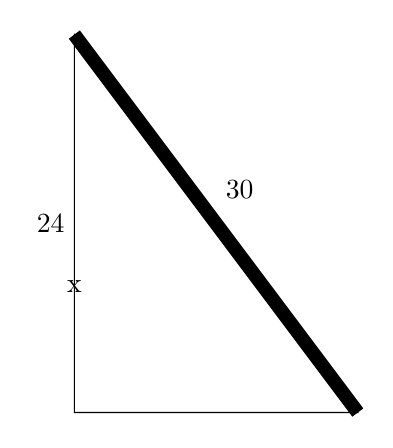
\begin{tikzpicture}[baseline=(current bounding box.north), scale = 2]
    \coordinate (A) at (0,0);
    \coordinate (B) at (1.8,0);
    \coordinate (C) at (0,2.4);

    \draw (A) -- (B) -- (C) --cycle;
    \draw[line width=5pt] (B) -- (C);
    \node[left] at (0,1.2) {24};
    \node[above right] at (0.9,1.3) {30};
    \node[below] at (0,0.9) {x};
    
\end{tikzpicture}
\end{minipage}
\par
\subsection{Pi}
Dadas las instrucciones del PDF proporcionado, los frijoles puestos en el circulo, se acomodaban mejor en el cuadrado de 8 cm
\begin{center}
    \begin{tabular}{cc}
        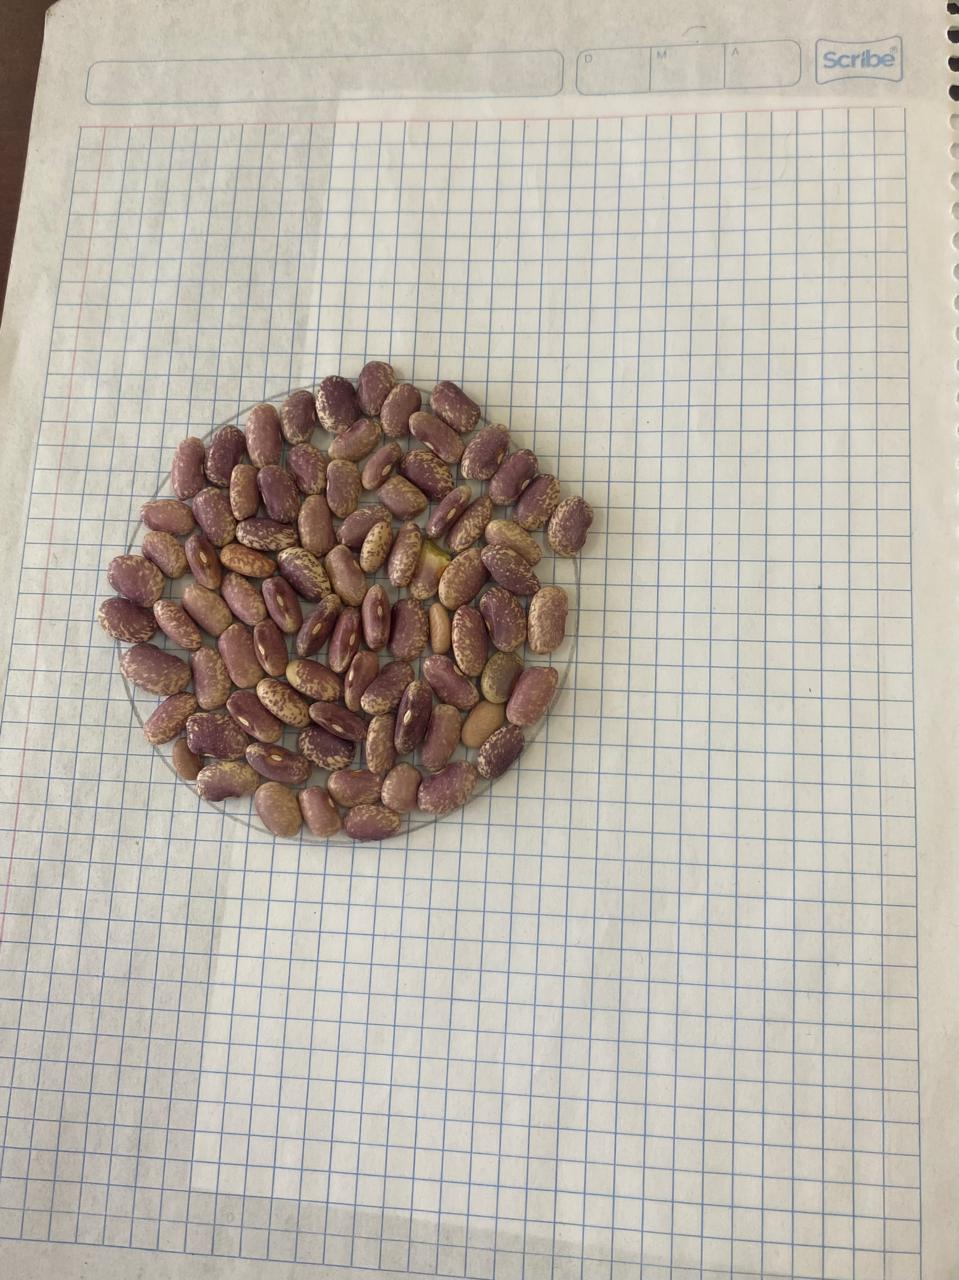
\includegraphics[scale=0.15]{clase22/frijoles-circulares.jpeg} & 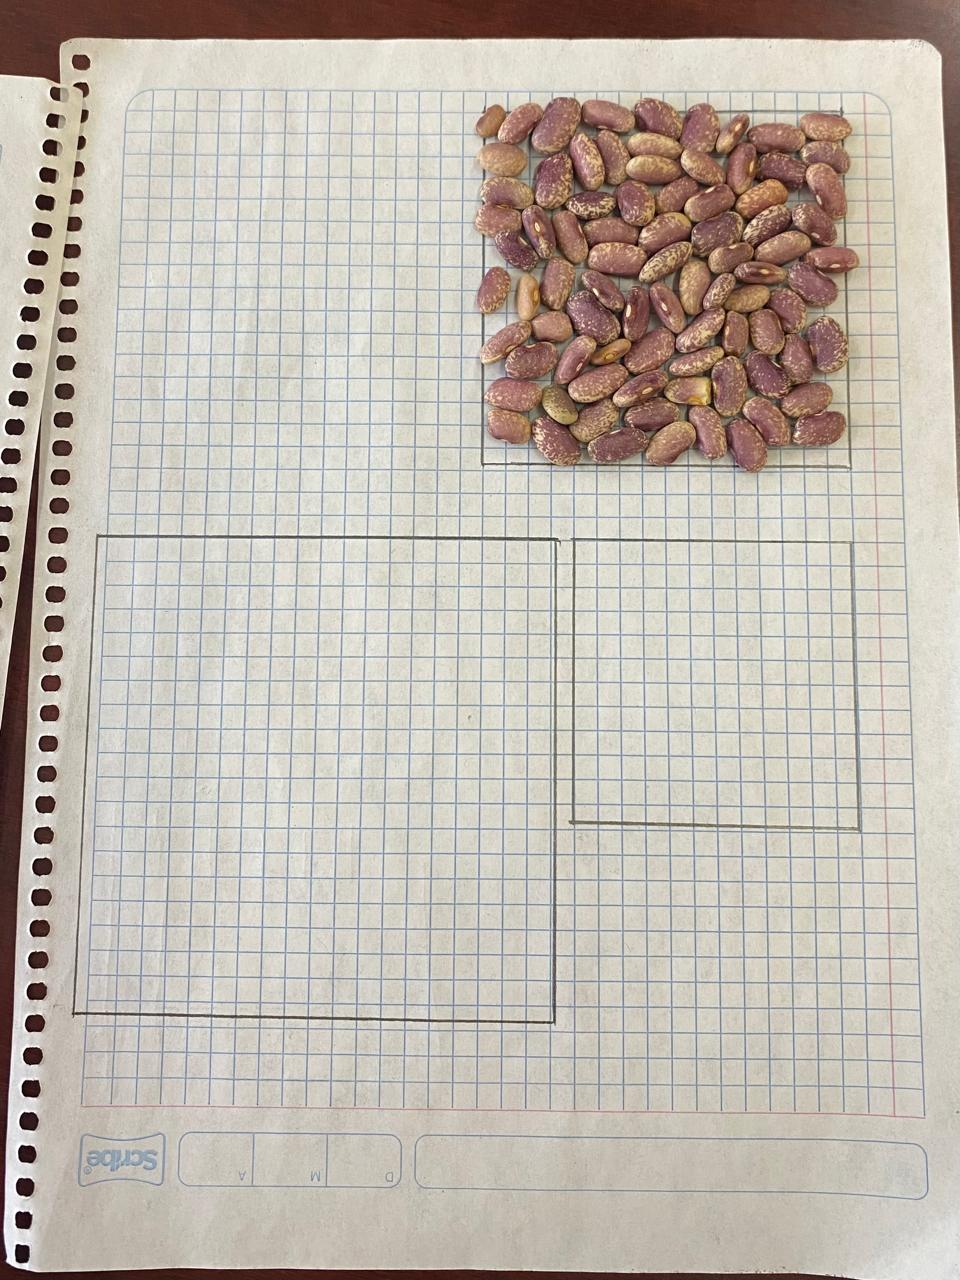
\includegraphics[scale=0.15]{clase22/frijoles-cuadrados.jpeg}
    \end{tabular}
\end{center}
Tenemos que el área del circulo es $A=\pi r^{2} = \pi 4.5^{2} \approx 63.617551$ mientras que $A_{c} = 8\cdot8 = 64$, con $A_{c}$ como área del cuadrado.\\

¿Cuál fue el cuadrado que se ajustó mejor al área del círculo? R: El cuadrado con medida de 8cm de lado\\
Sabiendo que el área del círculo es $A = \pi r^{2}$ y que el área del cuadrado se calcula $A_{c} = l \cdot l $¿Podrías calcular el valor de $\pi$?, ¿Cuál fue el valor que obtuviste para $\pi$? R: Despejando $\pi$ tenemos $\pi = \frac{63.617551}{4.5^{2}} \approx 3.141607$\\

¿Cómo podrías mejorar el método para calcular $\pi$? R: siguiendo la misma idea. Dado que el área del cuadrado es mayor a la del circulo sería disminuyendo el valor del lado del cuadrado para obtener una aproximación después del punto en las milesimas, pero también ocupando algun grano que puede rellenar mejor tanto el área del cuadrado y del círculo dejando la menor cantidad de espacio.
\subsection{Proporción aurea}
Con las instrucciones proporcionadas en el PDF trazamos una curva de Duero, aunque fue un martirio en cuanto los segmentos y arcos de circunferencia se hacían más cortos
\begin{center}
    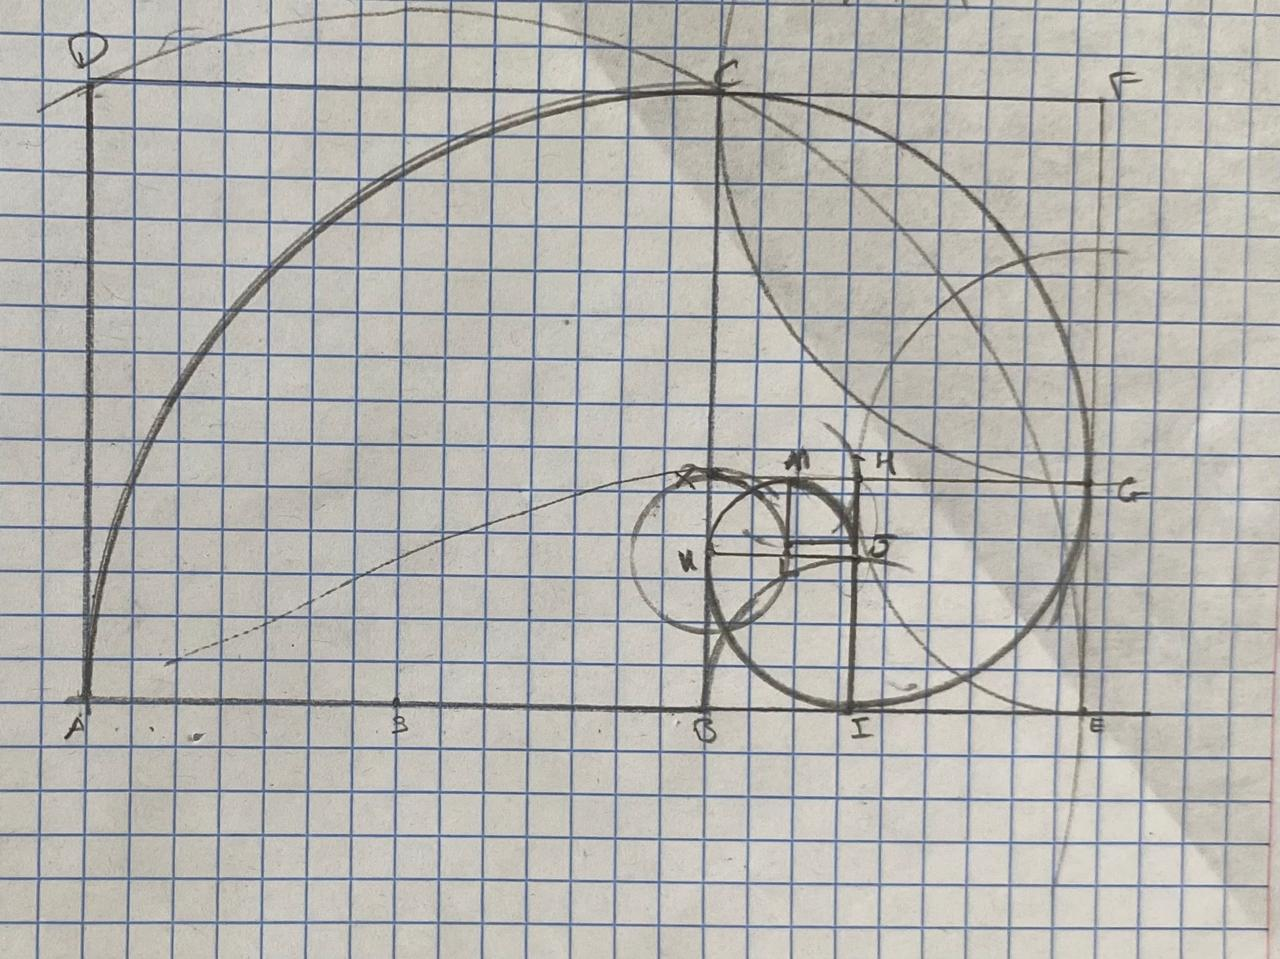
\includegraphics[scale=0.15]{clase22/proporcion-aurea.jpeg}
\end{center}